\documentclass[oneside,10pt]{book}

\usepackage{cdtBook}
\usepackage{usecases}
\usepackage[table,xcdraw]{xcolor}
\usepackage{tabularx}

%Espacios
\newcommand\tab[1][1cm]{\hspace*{#1}}

\title{Módulo de torneos de fútbol }
\subtitle{GPA-P1-E1-Guion de Pruebas de Aceptación}
\author{Autores: \\Aguilera Ramírez Rubén Omar \\ Altamirano Lara Jesús David \\ Arredondo Basurto Edgar Rodrigo \\ Fernández Quiñones Isaac \\ Flores Mejía Irving Alan \\ Galicia Vargas Gerardo \\ Hernández Gómez Ricardo Neftali \\ Hernández Quintero Victor \\ Landa Aguirre Rafael\\ Morales García Miguel Ángel \\ Mundo López Alejandro Edgar \\ \\}
\organization{Escuela Superior de Cómputo, IPN}

%%%%%%%%%%%%%%%%%%%%%%%%%%%%%%%%%%%%%%%%%%%%%%%%%%%%%%%%%%%%%%%%
\begin{document}

\maketitle

\begin{table}[]
\centering
\label{my-label}
\begin{tabularx}{\textwidth}{ X l X X }
\multicolumn{4}{c}{\cellcolor[HTML]{CBCEFB}Proyecto}                                                                                         \\ \hline
\multicolumn{1}{|X|}{Clave} & \multicolumn{1}{X|}{Nombre}                      & \multicolumn{1}{X|}{Etapa}   & \multicolumn{1}{l|}{Uso}     \\ \hline
\multicolumn{1}{|X|}{MTF}   & \multicolumn{1}{l|}{Módulo de Torneos de Fútbol} & \multicolumn{1}{X|}{Inicial} & \multicolumn{1}{X|}{Interno} \\ \hline
\end{tabularx}
\end{table}

\begin{table}[]
\centering
\label{my-label}
\begin{tabularx}{\textwidth}{ X l X X }
\multicolumn{4}{c}{\cellcolor[HTML]{CBCEFB}Documento}                                                                                         \\ \hline
\multicolumn{1}{|X|}{Clave} 		& \multicolumn{1}{X|}{Nombre}                      		& \multicolumn{1}{X|}{Versión}   	& \multicolumn{1}{l|}{Fecha}     \\ \hline
\multicolumn{1}{|X|}{GPA-P1-E1}   	& \multicolumn{1}{l|}{Guion de pruebas de aceptación} 	& \multicolumn{1}{X|}{1.0} 		& \multicolumn{1}{X|}{23 de abril de 2017} \\ \hline
\end{tabularx}
\end{table}

\begin{table}[]
\centering
\label{my-label}
\begin{tabularx}{\textwidth}{ X l X X }
\multicolumn{4}{c}{\cellcolor[HTML]{CBCEFB}Elementos entregados}                                                                                         \\ \hline
\multicolumn{1}{|X|}{Clave} 		& \multicolumn{1}{X|}{Nombre}                      		& \multicolumn{1}{X|}{Versión}   	& \multicolumn{1}{l|}{Aprobado}     \\ \hline
\multicolumn{1}{|X|}{GPA-P1-E1}   	& \multicolumn{1}{l|}{Guion de pruebas de aceptación} 	& \multicolumn{1}{X|}{1.0} 		& \multicolumn{1}{X|}{ } \\ \hline
\end{tabularx}
\end{table}

\begin{table}[]
\centering
\label{my-label}
\begin{tabularx}{\textwidth}{ X X X X }
\multicolumn{4}{c}{\cellcolor[HTML]{CBCEFB}Documentos relacionados}                                                                                         \\ \hline
\multicolumn{1}{|X|}{Clave} 		& \multicolumn{1}{X|}{Nombre}                      		& \multicolumn{1}{X|}{Versión}   	& \multicolumn{1}{X|}{Fecha}     \\ \hline
\multicolumn{1}{|X|}{Documento de análisis}   	& \multicolumn{1}{X|}{Análisis del sistema para la Liga de fútbol: El bolillo de ESCOM} 	& \multicolumn{1}{X|}{2.0} 		& \multicolumn{1}{X|}{23 de abril de 2017} \\ \hline
\end{tabularx}
\end{table}

\begin{table}[]
\centering
\label{my-label}
\begin{tabularx}{\textwidth}{ X }
\multicolumn{1}{c}{\cellcolor[HTML]{CBCEFB}Observaciones}                                                                                         \\ \hline
\multicolumn{1}{ |X| }{ } \\
\multicolumn{1}{ |X| }{ } \\
\multicolumn{1}{ |X| }{ } \\
\multicolumn{1}{ |X| }{ } \\
\multicolumn{1}{ |X| }{ } \\
\multicolumn{1}{ |X| }{ } \\
\multicolumn{1}{ |X| }{ } \\
\multicolumn{1}{ |X| }{ }                                                                                        
\\ \hline
\end{tabularx}
\end{table}

\begin{table}[]
\centering
\label{my-label}
\begin{tabularx}{\textwidth}{ X X X }
\multicolumn{3}{c}{\cellcolor[HTML]{CBCEFB}Firmas}                                                                                         \\ \hline
\multicolumn{1}{|X|}{ } & \multicolumn{1}{X|}{ } & \multicolumn{1}{X|}{ } \\
\multicolumn{1}{|c|}{Elaboró} 		& \multicolumn{1}{c|}{Supervisó}                   		& \multicolumn{1}{c|}{Aprobó} \\
\multicolumn{1}{|X|}{ } & \multicolumn{1}{X|}{ } & \multicolumn{1}{X|}{ } \\
\multicolumn{1}{|X|}{ } & \multicolumn{1}{X|}{ } & \multicolumn{1}{X|}{ } \\
\multicolumn{1}{|X|}{ } & \multicolumn{1}{X|}{ } & \multicolumn{1}{X|}{ } \\
\multicolumn{1}{|X|}{ } & \multicolumn{1}{X|}{ } & \multicolumn{1}{X|}{ } \\ \hline
\multicolumn{1}{|c|}{Galicia Vargas Gerardo}   	& \multicolumn{1}{c|}{Aguilera Ramirez Omar} 	& \multicolumn{1}{c|}{Maldonado Castillo Idalia} 	\\
\multicolumn{1}{|c|}{Responsable}   	& \multicolumn{1}{c|}{ } 	& \multicolumn{1}{c|}{ } \\
\multicolumn{1}{|X|}{ } & \multicolumn{1}{X|}{ } & \multicolumn{1}{X|}{ } \\ \hline
\end{tabularx}
\end{table}

\thispagestyle{empty}

\frontmatter
\tableofcontents

\mainmatter

%=========================================================
%=========================================================
\chapter{Descripción de las pruebas}

%=========================================================
\section{Propósito de las pruebas}

	Verificar la funcionalidad de los casos de uso correspondientes al registro de un Representante, gestión de jugadores y equipos de un Representante, como parte del Módulo de torneos, además de las funciones necesarias para acceder a tales casos de uso.

%=========================================================
\section{Alcance}

	Las pruebas contenidas en el presente instrumento están orientadas a verificar que el entregable permita:

\begin{itemize}
\item Crear una cuenta de usuario Representante.
\item Iniciar sesión como Representante.
\item Gestionar información de jugadores.
\item Gestionar equipos.
\end{itemize}

%=========================================================
\section{Elementos involucrados en las pruebas}

	Se verificará la funcionalidad de las trayectorias principales y alternativas de los siguientes Casos de Uso:
\begin{itemize}
\item \textbf{CU1} Gestionar información de jugadores.
	\begin{itemize}
	\item \textbf{CU1.1} Registrar jugador.
	\item \textbf{CU1.2} Eliminar jugador.
	\item \textbf{CU1.3} Actualizar información de un jugador.
	\end{itemize}
\item \textbf{CU2} Gestionar equipo.
	\begin{itemize}
	\item \textbf{CU2.1} Crear equipo.
	\item \textbf{CU2.2} Eliminar equipo.
	\item \textbf{CU2.3} Actualizar equipo.
	\item \textbf{CU2.4} Ver plantilla del equipo.
	\end{itemize}
\item \textbf{CU6} Iniciar sesión.
\item \textbf{CU7} Registrar Representante.
\end{itemize}

	Se verificará la redacción de los mensajes: MSG1.0, MSG1.1, MSG1.2, MSG1.3, MSG1.3.1, MSG1.3.2, MSG1.3.3, MSG1.3.4, MSG1.4, MSG1.4.1, MSG1.5, MSG1.5.1, MSG1.8, MSG2.3, MSG2.3.1, MSG2.4, MSG6.1, MSG1.3.1, MSG7.0, MSG1.3.1, MSG7.2, MSG7.3, MSG7.8, MSG1.3.1 y MSG10.2.\\
	
	Se verificará la distribución, redacción y estilos de las pantallas:

\begin{itemize}
\item \textbf{IU0} Pantalla principal.
\item \textbf{IU1.0} Pantalla de inicio del representante.
\item \textbf{IU1.1} Modal para registrar jugador.
\item \textbf{IU1.2} Pantalla emergente para eliminar jugador.
\item \textbf{IU1.3} Modal para actualizar datos de jugador.
\item \textbf{IU2.1} Modal para crear equipo.
\item \textbf{IU2.2} Pantalla emergente para eliminar equipo.
\item \textbf{IU2.3} Modal para actualizar equipo.
\item \textbf{IU2.4} Modal para ver plantilla de jugadores.
\item \textbf{IU6.0} Pantalla de inicio de sesión.
\item \textbf{IU7.0} Pantalla de registro del representante.
\end{itemize}	

%=========================================================
\section{Requisitos para correr las pruebas}

Para el uso del presente instrumento se requerirán los siguientes elementos:

\begin{itemize}
	\item El equipo desde el que se correrán las pruebas debe cumplir con las características de software y hardware del \textbf{Equipo cliente} definidas en el Documento de análisis del sistema.
	\item El \textbf{Equipo cliente} deberá tener acceso al servidor seleccionado para la ejecución de las pruebas.
\end{itemize}


\begin{tabularx}{\textwidth}{ l X }
\hline
\multicolumn{1}{l}{\cellcolor[HTML]{CBCEFB}Datos de la prueba} & \multicolumn{1}{X}{\cellcolor[HTML]{CBCEFB} }     \\ \hline
\multicolumn{1}{|l|}{Tipo de prueba}   & \multicolumn{1}{X|}{ $\square$Complementaria $\square$Completa} \\ \hline
\multicolumn{1}{|l|}{Sistema}   & \multicolumn{1}{X|}{ } \\ \hline
\multicolumn{1}{|l|}{Fecha de aplicación}   & \multicolumn{1}{X|}{ } \\ \hline
\multicolumn{1}{|l|}{Hora de inicio}   & \multicolumn{1}{X|}{ } \\ \hline
\multicolumn{1}{|l|}{Hora de término}   & \multicolumn{1}{X|}{ } \\ \hline
\multicolumn{1}{|l|}{Nombre del líder de pruebas}   & \multicolumn{1}{X|}{ } \\ \hline
\multicolumn{1}{|l|}{Nombre tester}   & \multicolumn{1}{X|}{ } \\ \hline
\end{tabularx}

%=========================================================
\section{Equipo de pruebas}

\begin{tabularx}{\textwidth}{ l X }
\hline
\multicolumn{1}{l}{\cellcolor[HTML]{CBCEFB}Datos de la prueba} & \multicolumn{1}{X}{\cellcolor[HTML]{CBCEFB} }     \\ \hline
\multicolumn{1}{|l|}{Equipo servidor de prueba}   & \multicolumn{1}{X|}{ Apache Tomcat 8.0.32 } \\ \hline
\multicolumn{1}{|l|}{Equipo cliente de prueba}   & \multicolumn{1}{X|}{ } \\ \hline
\multicolumn{1}{|l|}{Navegador cliente de prueba}   & \multicolumn{1}{X|}{ Mozilla Firefox o Google Chrome} \\ \hline
\end{tabularx}
\\
%=========================================================
\section{Documento de referencia}

Documento de \textbf{Análisis del sistema para la Liga de fútbol: El bolillo de ESCOM}. \\

%=========================================================
\section{Configuración de pruebas}

\begin{itemize}
\item En el navegador, Mozilla Firefox, desactive el bloqueo de ventanas emergentes.
\item Ajuste el zoom de su navegador al 100\% y maximice la ventana.
\end{itemize}

Al ingresar a la URL \textit{http://localhost:8080/TorneoFutbol/}, de la página principal, deben mostrarse los botones e iconos de la imagen que se muestra a continuación: \\ \\
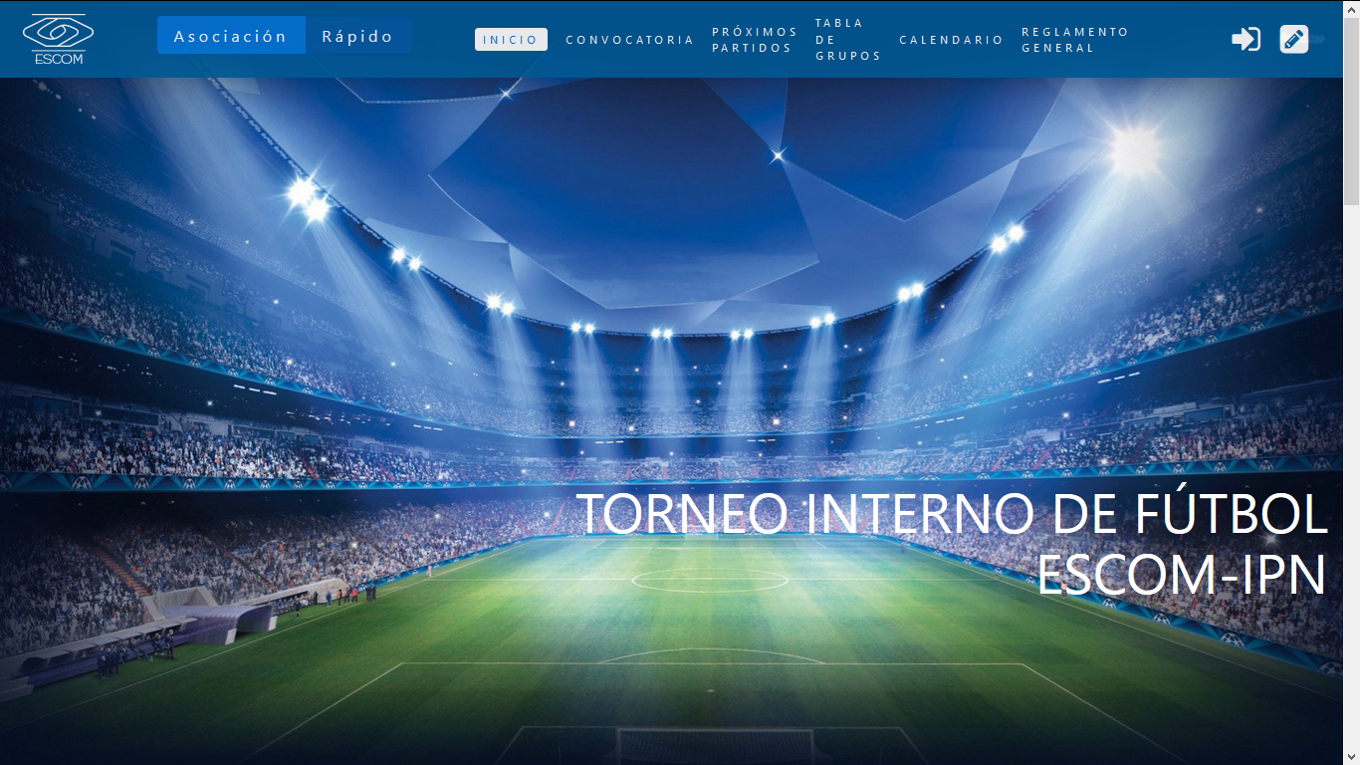
\includegraphics[scale=.5]{images/index_sample}

%=========================================================
%=========================================================
\chapter{Ejecución de pruebas}

%=========================================================
\section{Checklist}

\begin{itemize}
\item $\square$ Guion de pruebas
\item $\square$ Lápiz
\item $\square$ El equipo cliente de pruebas cumple con las características especificadas.
\item $\square$ El equipo servidor de pruebas cumple con las características especificadas.
\item $\square$ El acceso a la aplicación está activo.
\item $\square$ El Documento de análisis.
\end{itemize}

%=========================================================
\section{Instrucciones}

Para ejecutar las pruebas correspondientes a este módulo: \\

1. Verifique que el servidor de aplicaciones esté corriendo y contenga la versión adecuada del módulo a probar. \\

%=========================================================
\newpage
\subsection{P1-E1-CP1: Prueba de funcionalidad, Verificación de pantallas}

\begin{tabularx}{\textwidth}{ l l l X }
\multicolumn{4}{c}{\cellcolor[HTML]{9B9B9B}\textbf{Sistema: MTF}}                                                                                     \\
\multicolumn{4}{c}{\cellcolor[HTML]{EFEFEF}\textbf{P1-E1-CP1 Prueba de Funcionalidad, Verificación de Pantallas.}}                                    \\ \hline
\multicolumn{1}{|l|}{Instrucción}                               & \multicolumn{1}{l|}{Aprobada} & \multicolumn{1}{l|}{No aprobada} & \multicolumn{1}{X|}{Observaciones} \\ \hline
\multicolumn{1}{|l|}{1. Ingrese, desde el navegador Mozilla Firefox, a la URL:} & \multicolumn{1}{l|}{}   & \multicolumn{1}{l|}{}   & \multicolumn{1}{X|}{}              \\
\multicolumn{1}{|l|}{http://localhost:8080/TorneoFutbol/} & \multicolumn{1}{l|}{ } & \multicolumn{1}{l|}{ } & \multicolumn{1}{X|}{ } \\ 
\multicolumn{1}{|l|}{ } & \multicolumn{1}{l|}{ } & \multicolumn{1}{l|}{ } & \multicolumn{1}{X|}{ } \\ \hline
\multicolumn{4}{|l|}{Evalúe la interfaz \textbf{IU0 Pantalla principal}. $\square$CSS, $\square$Ortografía, $\square$Alineación, $\square$Espacios, $\square$Iconografía,}                        \\
\multicolumn{4}{|l|}{$\square$Tamaño de campos}                        \\ \hline
\multicolumn{1}{|l|}{2. En la parte superior derecha de la pantalla actual, dé clic} & \multicolumn{1}{l|}{}   & \multicolumn{1}{l|}{ }   & \multicolumn{1}{X|}{}              \\
\multicolumn{1}{|l|}{sobre el icono 
\includegraphics[scale=.3]{images/signin}.} & \multicolumn{1}{l|}{ } & \multicolumn{1}{l|}{ } & \multicolumn{1}{X|}{ } \\
\multicolumn{1}{|l|}{Recorra el contenido de la pantalla, por medio del \textit{scroll}.} & \multicolumn{1}{l|}{ } & \multicolumn{1}{l|}{ } & \multicolumn{1}{X|}{ } \\ \hline
\multicolumn{4}{|l|}{Evalúe la interfaz \textbf{IU7.0 Pantalla de registro del Representante}. $\square$CSS, $\square$Ortografía, $\square$Alineación,}                        \\
\multicolumn{4}{|l|}{$\square$Espacios, $\square$Iconografía, $\square$Tamaño de campos}                        \\ \hline
\multicolumn{1}{|l|}{3. En la parte superior derecha de la pantalla actual, dé clic} & \multicolumn{1}{l|}{}   & \multicolumn{1}{l|}{}   & \multicolumn{1}{X|}{}              \\
\multicolumn{1}{|l|}{sobre el icono 
\includegraphics[scale=.3]{images/login}.} & \multicolumn{1}{l|}{ } & \multicolumn{1}{l|}{ } & \multicolumn{1}{X|}{ } \\
\multicolumn{1}{|l|}{ } & \multicolumn{1}{l|}{ } & \multicolumn{1}{l|}{ } & \multicolumn{1}{X|}{ } \\ \hline
\multicolumn{4}{|l|}{Evalúe la interfaz \textbf{IU6.0 Pantalla de inicio de sesión}. $\square$CSS, $\square$Ortografía, $\square$Alineación, $\square$Espacios,}                        \\
\multicolumn{4}{|l|}{$\square$Iconografía, $\square$Tamaño de campos}                        \\ \hline
\multicolumn{1}{|l|}{4. Introduzca la dirección de correo: \textit{isaac$@$gmail.com}.} & \multicolumn{1}{l|}{}   & \multicolumn{1}{l|}{}   & \multicolumn{1}{X|}{}              \\
\multicolumn{1}{|l|}{Introduzca la contraseña: \textit{isaacroot1}.} & \multicolumn{1}{l|}{}   & \multicolumn{1}{l|}{}   & \multicolumn{1}{X|}{}              \\ 
\multicolumn{1}{|l|}{Presione el botón \IUbutton{Iniciar sesión}.} & \multicolumn{1}{l|}{}   & \multicolumn{1}{l|}{}   & \multicolumn{1}{X|}{}              \\ \hline
\multicolumn{4}{|l|}{Evalúe la interfaz \textbf{IU1.0 Pantalla de inicio del representante}. $\square$CSS, $\square$Ortografía, $\square$Alineación,}                        \\
\multicolumn{4}{|l|}{$\square$Espacios, $\square$Iconografía, $\square$Tamaño de campos}                        \\ \hline
\multicolumn{1}{|l|}{5. En la pantalla actual, presione el botón 
\includegraphics[scale=.3]{images/add}, de la} & \multicolumn{1}{l|}{}   & \multicolumn{1}{l|}{}   & \multicolumn{1}{X|}{}              \\
\multicolumn{1}{|l|}{sección \textit{Mis Jugadores}.} & \multicolumn{1}{l|}{ } & \multicolumn{1}{l|}{ } & \multicolumn{1}{X|}{ } \\ 
\multicolumn{1}{|l|}{ } & \multicolumn{1}{l|}{ } & \multicolumn{1}{l|}{ } & \multicolumn{1}{X|}{ } \\ \hline
\multicolumn{4}{|l|}{Evalúe la interfaz \textbf{IU1.1 Modal para registrar jugador}. $\square$CSS, $\square$Ortografía, $\square$Alineación,}                        \\
\multicolumn{4}{|l|}{$\square$Espacios, $\square$Iconografía, $\square$Tamaño de campos}                        \\ \hline

\multicolumn{1}{|l|}{6. Cierre la \textbf{IU1.1 Modal para registrar jugador}.} & \multicolumn{1}{l|}{}   & \multicolumn{1}{l|}{}   & \multicolumn{1}{X|}{}              \\
\multicolumn{1}{|l|}{Dé clic sobre el icono 
\includegraphics[scale=.3]{images/edit} de alguno de los jugadores} & \multicolumn{1}{l|}{ } & \multicolumn{1}{l|}{ } & \multicolumn{1}{X|}{ } \\ 
\multicolumn{1}{|l|}{registrados en la sección \textit{Mis Jugadores}.} & \multicolumn{1}{l|}{ } & \multicolumn{1}{l|}{ } & \multicolumn{1}{X|}{ } \\ \hline
\multicolumn{4}{|l|}{Evalúe la interfaz \textbf{IU1.3 Modal para actualizar datos de jugador}. $\square$CSS, $\square$Ortografía, $\square$Alineación,}                        \\
\multicolumn{4}{|l|}{$\square$Espacios, $\square$Iconografía, $\square$Tamaño de campos}                        \\ \hline

\multicolumn{1}{|l|}{7. Cierre el \textbf{IU1.3 Modal para actualizar datos de jugador}.} & \multicolumn{1}{l|}{}   & \multicolumn{1}{l|}{}   & \multicolumn{1}{X|}{}              \\
\multicolumn{1}{|l|}{Dé clic sobre el icono 
\includegraphics[scale=.3]{images/eliminate} de alguno de los jugadores} & \multicolumn{1}{l|}{ } & \multicolumn{1}{l|}{ } & \multicolumn{1}{X|}{ } \\ 
\multicolumn{1}{|l|}{registrados en la sección \textit{Mis Jugadores}.} & \multicolumn{1}{l|}{ } & \multicolumn{1}{l|}{ } & \multicolumn{1}{X|}{ } \\ \hline
\multicolumn{4}{|l|}{Evalúe la interfaz \textbf{IU1.2 Pantalla emergente para eliminar jugador}. $\square$CSS, $\square$Ortografía, $\square$Alineación,}                        \\
\multicolumn{4}{|l|}{$\square$Espacios, $\square$Iconografía, $\square$Tamaño de campos}                        \\ \hline
\end{tabularx}

\begin{tabularx}{\textwidth}{ l l l X } \\
\hline
\multicolumn{1}{|l|}{Instrucción}                               & \multicolumn{1}{l|}{Aprobada} & \multicolumn{1}{l|}{No aprobada} & \multicolumn{1}{X|}{Observaciones} \\ \hline
\multicolumn{1}{|l|}{8. Cierre la \textbf{IU1.2 Pantalla emergente para eliminar jugador}.} & \multicolumn{1}{l|}{}   & \multicolumn{1}{l|}{}   & \multicolumn{1}{X|}{}              \\
\multicolumn{1}{|l|}{Con el \textit{scroll}, diríjase a la parte inferior de la pantalla y presione} & \multicolumn{1}{l|}{ } & \multicolumn{1}{l|}{ } & \multicolumn{1}{X|}{ } \\ 
\multicolumn{1}{|l|}{el botón 
\includegraphics[scale=.3]{images/add}, de la sección \textit{Mis Equipos}.} & \multicolumn{1}{l|}{ } & \multicolumn{1}{l|}{ } & \multicolumn{1}{X|}{ } \\ \hline
\multicolumn{4}{|l|}{Evalúe la interfaz \textbf{IU2.1 Modal para crear equipo}. $\square$CSS, $\square$Ortografía, $\square$Alineación,}                        \\
\multicolumn{4}{|l|}{$\square$Espacios, $\square$Iconografía, $\square$Tamaño de campos}                        \\ \hline

\multicolumn{1}{|l|}{9. Cierre la \textbf{IU2.1 Modal para crear equipo}.} & \multicolumn{1}{l|}{}   & \multicolumn{1}{l|}{}   & \multicolumn{1}{X|}{}              \\
\multicolumn{1}{|l|}{Dé clic sobre el icono 
\includegraphics[scale=.3]{images/visualize} del equipo registrado, \textit{ESCOM 1}.} & \multicolumn{1}{l|}{ } & \multicolumn{1}{l|}{ } & \multicolumn{1}{X|}{ } \\ 
\multicolumn{1}{|l|}{ } & \multicolumn{1}{l|}{ } & \multicolumn{1}{l|}{ } & \multicolumn{1}{X|}{ } \\ \hline
\multicolumn{4}{|l|}{Evalúe la interfaz \textbf{IU2.4 Modal para ver plantilla de jugadores}. $\square$CSS, $\square$Ortografía, $\square$Alineación,}                        \\
\multicolumn{4}{|l|}{$\square$Espacios, $\square$Iconografía, $\square$Tamaño de campos}                        \\ \hline

\multicolumn{1}{|l|}{10. Cierre el \textbf{IU2.4 Modal para ver plantilla de jugadores}.} & \multicolumn{1}{l|}{}   & \multicolumn{1}{l|}{}   & \multicolumn{1}{X|}{}              \\
\multicolumn{1}{|l|}{Dé clic sobre el icono 
\includegraphics[scale=.3]{images/edit} del equipo registrado.} & \multicolumn{1}{l|}{ } & \multicolumn{1}{l|}{ } & \multicolumn{1}{X|}{ } \\ 
\multicolumn{1}{|l|}{ } & \multicolumn{1}{l|}{ } & \multicolumn{1}{l|}{ } & \multicolumn{1}{X|}{ } \\ \hline
\multicolumn{4}{|l|}{Evalúe la interfaz \textbf{IU2.3 Modal para actualizar equipo}. $\square$CSS, $\square$Ortografía, $\square$Alineación,}                        \\
\multicolumn{4}{|l|}{$\square$Espacios, $\square$Iconografía, $\square$Tamaño de campos}                        \\ \hline

\multicolumn{1}{|l|}{11. Cierre el \textbf{IU2.3 Modal para actualizar equipo}.} & \multicolumn{1}{l|}{}   & \multicolumn{1}{l|}{}   & \multicolumn{1}{X|}{}              \\
\multicolumn{1}{|l|}{Dé clic sobre el icono 
\includegraphics[scale=.3]{images/eliminate} del equipo registrado.} & \multicolumn{1}{l|}{ } & \multicolumn{1}{l|}{ } & \multicolumn{1}{X|}{ } \\ 
\multicolumn{1}{|l|}{ } & \multicolumn{1}{l|}{ } & \multicolumn{1}{l|}{ } & \multicolumn{1}{X|}{ } \\ \hline
\multicolumn{4}{|l|}{Evalúe la interfaz \textbf{IU2.2 Pantalla emergente para eliminar equipo}. $\square$CSS, $\square$Ortografía, $\square$Alineación,}                        \\
\multicolumn{4}{|l|}{$\square$Espacios, $\square$Iconografía, $\square$Tamaño de campos}                        \\ \hline
\end{tabularx}

\begin{tabularx}{\textwidth}{ X }
\multicolumn{1}{X}{\cellcolor[HTML]{9B9B9B}\textbf{Observaciones}} \\ \hline
\multicolumn{1}{|l|}{ }	\\
\multicolumn{1}{|l|}{ }	\\
\multicolumn{1}{|l|}{ }	\\
\multicolumn{1}{|l|}{ }	\\
\multicolumn{1}{|l|}{ }	\\
\multicolumn{1}{|l|}{ }	\\
\multicolumn{1}{|l|}{ }	\\
\multicolumn{1}{|l|}{ }	\\
\multicolumn{1}{|l|}{ }	\\
\multicolumn{1}{|l|}{ }	\\
\multicolumn{1}{|l|}{ }	\\
\multicolumn{1}{|l|}{ }	\\
\multicolumn{1}{|l|}{ }	\\
\multicolumn{1}{|l|}{ }	\\ \hline
\end{tabularx}
%=========================================================
\newpage
\subsection{P1-E1-CP2: Prueba de funcionalidad, caso Registrar Representante}

\begin{tabularx}{\textwidth}{ X l l X }
\multicolumn{4}{c}{\cellcolor[HTML]{9B9B9B}\textbf{Sistema: MTF}}                                                                                     \\
\multicolumn{4}{c}{\cellcolor[HTML]{EFEFEF}\textbf{P1-E1-CP2 Prueba de Funcionalidad, caso Registrar Representante.}}                                    \\ \hline
\multicolumn{1}{|X|}{Instrucciones y preguntas}                               & \multicolumn{1}{l|}{Sí} & \multicolumn{1}{l|}{No} & \multicolumn{1}{X|}{Observaciones} \\ \hline
\multicolumn{4}{|l|}{1. Ingrese, desde el navegador Mozilla Firefox, a la URL: http://localhost:8080/TorneoFutbol/}              \\ \hline
\multicolumn{1}{|X|}{1.1 ¿El sistema mostró la \textbf{IU0 Pantalla principal}?} & \multicolumn{1}{l|}{}   & \multicolumn{1}{l|}{}   & \multicolumn{1}{X|}{}              \\ \hline
\multicolumn{4}{|l|}{2. En la parte superior derecha de la pantalla actual, presione sobre el icono 
\includegraphics[scale=.3]{images/signin}, correspondiente al \textbf{CU7}}              \\
\multicolumn{4}{|l|}{\textbf{Registrar representante}.}              \\ \hline
\multicolumn{1}{|X|}{2.1 ¿El sistema mostró la \textbf{IU7.0 Pantalla de registro del representante}?} & \multicolumn{1}{l|}{}   & \multicolumn{1}{l|}{}   & \multicolumn{1}{X|}{}              \\ \hline
\multicolumn{4}{|l|}{3. Con el \textit{scroll}, desplácese a la parte inferior de la pantalla y presione sobre el botón \IUbutton{Registrar}.}              \\ \hline
\multicolumn{1}{|X|}{3.1. ¿El sistema mostró el \textbf{MSG10.2 ''Este campo es obligatorio''} bajo todos los campos, excepto el de fotografía?} & \multicolumn{1}{l|}{}   & \multicolumn{1}{l|}{}   & \multicolumn{1}{X|}{}              \\ \hline
\multicolumn{1}{|X|}{3.2. ¿El sistema mostró el \textbf{MSG1.3.4 ''Este campo es obligatorio. Selecciona una foto de perfil''} bajo el campo de fotografía?} & \multicolumn{1}{l|}{}   & \multicolumn{1}{l|}{}   & \multicolumn{1}{X|}{}              \\ \hline

\multicolumn{4}{|l|}{4. Introduzca el nombre: \textit{123}.}              \\
\multicolumn{4}{|l|}{Introduzca el apellido paterno: \textit{123}.}              \\
\multicolumn{4}{|l|}{Introduzca el apellido materno: \textit{123}.}              \\
\multicolumn{4}{|l|}{Introduzca el teléfono: \textit{teléfono}.}              \\
\multicolumn{4}{|l|}{Introduzca el correo: \textit{correo}.}              \\
\multicolumn{4}{|l|}{Introduzca el número de boleta: \textit{*}.}              \\

\multicolumn{4}{|l|}{Cargue el archivo jpg: \textit{FotoPesada.jpg} (que se localiza en la misma dirección que el presente instrumento).}              \\

\multicolumn{4}{|l|}{Introduzca la contraseña: \textit{123}.}              \\
\multicolumn{4}{|l|}{Introduzca la confirmación de contraseña: \textit{contraseña}.}              \\

\multicolumn{4}{|l|}{Presione el botón \IUbutton{Registrar}.}              \\ \hline

\multicolumn{1}{|X|}{4.1. El sistema mostró los mensajes en los campos:} & \multicolumn{1}{l|}{}   & \multicolumn{1}{l|}{}   & \multicolumn{1}{X|}{}              \\
\multicolumn{1}{|X|}{\textit{Nombre(s)}: \textbf{MSG1.3 ''Este campo solo admite letras''}} & \multicolumn{1}{l|}{}   & \multicolumn{1}{l|}{}   & \multicolumn{1}{X|}{}              \\ \hline
\multicolumn{1}{|X|}{4.2. \textit{Apellido Paterno}: \textbf{MSG1.3 ''Este campo solo admite letras''}} & \multicolumn{1}{l|}{}   & \multicolumn{1}{l|}{}   & \multicolumn{1}{X|}{}              \\ \hline
\multicolumn{1}{|X|}{4.3. \textit{Apellido Materno}: \textbf{MSG1.3 ''Este campo solo admite letras''}} & \multicolumn{1}{l|}{}   & \multicolumn{1}{l|}{}   & \multicolumn{1}{X|}{}              \\ \hline
\multicolumn{1}{|X|}{4.4. \textit{Teléfono}: \textbf{MSG1.3.3 ''Escribe el número de teléfono con el formato: 5544332211''}} & \multicolumn{1}{l|}{}   & \multicolumn{1}{l|}{}   & \multicolumn{1}{X|}{}              \\ \hline
\multicolumn{1}{|X|}{4.5. \textit{Correo electrónico}: \textbf{MSG1.3.1 ''Escribe la dirección de correo electrónico con el formato alguien@example.com''}} & \multicolumn{1}{l|}{}   & \multicolumn{1}{l|}{}   & \multicolumn{1}{X|}{}              \\ \hline
\multicolumn{1}{|X|}{4.6. \textit{Número de boleta}: \textbf{MSG1.3.2 ''Este campo solo acepta valores alfanuméricos''}} & \multicolumn{1}{l|}{}   & \multicolumn{1}{l|}{}   & \multicolumn{1}{X|}{}              \\ \hline
\multicolumn{1}{|X|}{4.7. \textit{Fotografía}: \textbf{MSG7.8 ''Este campo no acepta imágenes mayores a 2M''}} & \multicolumn{1}{l|}{}   & \multicolumn{1}{l|}{}   & \multicolumn{1}{X|}{}              \\ \hline
\multicolumn{1}{|X|}{4.8. \textit{Contraseña}: \textbf{MSG7.2 ''Se requieren entre 8-30 caracteres''}} & \multicolumn{1}{l|}{}   & \multicolumn{1}{l|}{}   & \multicolumn{1}{X|}{}              \\ \hline

\end{tabularx}


\begin{tabularx}{\textwidth}{ X l l X }
\hline
\multicolumn{1}{|X|}{Pregunta}                               & \multicolumn{1}{l|}{Si} & \multicolumn{1}{l|}{No} & \multicolumn{1}{X|}{Observaciones} \\ \hline

\multicolumn{1}{|X|}{4.9. \textit{Confirmar contraseña}: \textbf{MSG7.3 ''Las contraseñas no coinciden''}} & \multicolumn{1}{l|}{}   & \multicolumn{1}{l|}{}   & \multicolumn{1}{X|}{}              \\ \hline

\multicolumn{4}{|l|}{5. Introduzca el nombre: \textit{Abraham}.}              \\
\multicolumn{4}{|l|}{Introduzca el apellido paterno: \textit{Rosas}.}              \\
\multicolumn{4}{|l|}{Introduzca el apellido materno: \textit{Pastrana}.}              \\
\multicolumn{4}{|l|}{Introduzca el teléfono: \textit{5548041600}.}              \\
\multicolumn{4}{|l|}{Introduzca el correo: \textit{ropa\_ab16$@$hotmail.com}.}              \\
\multicolumn{4}{|l|}{Introduzca el número de boleta: \textit{2015630140}.}              \\

\multicolumn{4}{|l|}{Cargue la fotografía (archivo jpg): \textit{FotoPerfil.jpg} (que se localiza en la misma dirección que el presente}              \\
\multicolumn{4}{|l|}{instrumento).}              \\


\multicolumn{4}{|l|}{Introduzca la contraseña: \textit{abrahamroot1}.}              \\
\multicolumn{4}{|l|}{Introduzca la confirmación de contraseña: \textit{abrahamroot1}.}              \\

\multicolumn{4}{|l|}{Presione el botón \IUbutton{Registrar}.}              \\ \hline

\multicolumn{1}{|X|}{5.1. ¿El sistema mostró el \textbf{MSG7.0 ''Registro exitoso. Se completó el registro exitosamente''}?} & \multicolumn{1}{l|}{}   & \multicolumn{1}{l|}{}   & \multicolumn{1}{X|}{}              \\ \hline
\multicolumn{1}{|X|}{5.2. ¿El sistema mostró la \textbf{IU6.0 Pantalla de inicio de sesión}?} & \multicolumn{1}{l|}{}   & \multicolumn{1}{l|}{}   & \multicolumn{1}{X|}{}              \\ \hline
\end{tabularx}

\begin{tabularx}{\textwidth}{ X }
\multicolumn{1}{X}{\cellcolor[HTML]{9B9B9B}\textbf{Observaciones}} \\ \hline
\multicolumn{1}{|l|}{ }	\\
\multicolumn{1}{|l|}{ }	\\
\multicolumn{1}{|l|}{ }	\\
\multicolumn{1}{|l|}{ }	\\
\multicolumn{1}{|l|}{ }	\\
\multicolumn{1}{|l|}{ }	\\
\multicolumn{1}{|l|}{ }	\\
\multicolumn{1}{|l|}{ }	\\
\multicolumn{1}{|l|}{ }	\\
\multicolumn{1}{|l|}{ }	\\
\multicolumn{1}{|l|}{ }	\\
\multicolumn{1}{|l|}{ }	\\
\multicolumn{1}{|l|}{ }	\\
\multicolumn{1}{|l|}{ }	\\ \hline
\end{tabularx}
%=========================================================
\newpage
\subsection{P1-E1-CP3: Prueba de funcionalidad, caso Iniciar sesión}

\begin{tabularx}{\textwidth}{ X l l X }
\multicolumn{4}{c}{\cellcolor[HTML]{9B9B9B}\textbf{Sistema: MTF}}                                                                                     \\
\multicolumn{4}{c}{\cellcolor[HTML]{EFEFEF}\textbf{P1-E1-CP3 Prueba de Funcionalidad, caso Iniciar sesión.}}                                    \\ \hline
\multicolumn{1}{|X|}{Pregunta}                               & \multicolumn{1}{l|}{Si} & \multicolumn{1}{l|}{No} & \multicolumn{1}{X|}{Observaciones} \\ \hline
\multicolumn{4}{|l|}{1. En la pantalla actual, \textbf{IU6.0 Pantalla de inicio de sesión},}              \\
\multicolumn{4}{|l|}{presione el botón \IUbutton{Iniciar sesión}.}              \\ \hline
\multicolumn{1}{|X|}{1.1. ¿El sistema mostró el mensaje \textbf{MSG10.2 ''Este campo es obligatorio''}, bajo cada uno de los campos del formulario?} & \multicolumn{1}{l|}{}   & \multicolumn{1}{l|}{}   & \multicolumn{1}{X|}{}              \\ \hline

\multicolumn{4}{|l|}{2. Introduzca la dirección de correo: \textit{correo}.}               \\
\multicolumn{4}{|l|}{Introduzca la contraseña: \textit{contraseña}.}               \\ 
\multicolumn{4}{|l|}{Presione el botón \IUbutton{Iniciar sesión}.}               \\ \hline
\multicolumn{1}{|X|}{2.1. ¿El sistema mostró el \textbf{MSG1.3.1 ''Escribe la dirección de correo electrónico con el formato alguien@example.com''}, bajo el campo del correo?} & \multicolumn{1}{l|}{}   & \multicolumn{1}{l|}{}   & \multicolumn{1}{X|}{}              \\ \hline

\multicolumn{4}{|l|}{3. Introduzca la dirección de correo: \textit{ropa\_ab16$@$hotmail.com}.}               \\
\multicolumn{4}{|l|}{Introduzca la contraseña: \textit{contraseña}.}               \\ 
\multicolumn{4}{|l|}{Presione el botón \IUbutton{Iniciar sesión}.}               \\ \hline
\multicolumn{1}{|X|}{3.1. ¿El sistema mostró el \textbf{MSG6.1 ''Correo y/o contraseña no son correctos''}?} & \multicolumn{1}{l|}{}   & \multicolumn{1}{l|}{}   & \multicolumn{1}{X|}{}              \\ \hline

\multicolumn{4}{|l|}{4. Introduzca el correo: \textit{ropa\_ab16$@$hotmail.com}.}               \\
\multicolumn{4}{|l|}{Introduzca la contraseña: \textit{abrahamroot1}.}               \\ 
\multicolumn{4}{|l|}{Presione el botón \IUbutton{Iniciar sesión}.}               \\ \hline
\multicolumn{1}{|X|}{4.1. ¿El sistema redirecciona a la \textbf{IU1.0 Pantalla de inicio del representante}?} & \multicolumn{1}{l|}{}   & \multicolumn{1}{l|}{}   & \multicolumn{1}{X|}{}              \\ \hline
\end{tabularx}

\begin{tabularx}{\textwidth}{ X }
\multicolumn{1}{X}{\cellcolor[HTML]{9B9B9B}\textbf{Observaciones}} \\ \hline
\multicolumn{1}{|l|}{ }	\\
\multicolumn{1}{|l|}{ }	\\
\multicolumn{1}{|l|}{ }	\\
\multicolumn{1}{|l|}{ }	\\
\multicolumn{1}{|l|}{ }	\\
\multicolumn{1}{|l|}{ }	\\
\multicolumn{1}{|l|}{ }	\\
\multicolumn{1}{|l|}{ }	\\
\multicolumn{1}{|l|}{ }	\\
\multicolumn{1}{|l|}{ }	\\
\multicolumn{1}{|l|}{ }	\\
\multicolumn{1}{|l|}{ }	\\
\multicolumn{1}{|l|}{ }	\\
\multicolumn{1}{|l|}{ }	\\ \hline
\end{tabularx}
%=========================================================
\newpage
\subsection{P1-E1-CP4: Prueba de funcionalidad, caso Registrar jugador}

\begin{tabularx}{\textwidth}{ X l l X }
\multicolumn{4}{c}{\cellcolor[HTML]{9B9B9B}\textbf{Sistema: MTF}}                                                                                     \\
\multicolumn{4}{l}{\cellcolor[HTML]{EFEFEF}\textbf{P1-E1-CP4: Prueba de funcionalidad, caso Registrar jugador}}                                    \\ \hline
\multicolumn{1}{|X|}{Pregunta}                               & \multicolumn{1}{l|}{Si} & \multicolumn{1}{l|}{No} & \multicolumn{1}{X|}{Observaciones} \\ \hline
\multicolumn{4}{|l|}{1. En la pantalla actual, \textbf{IU1.0 Pantalla de inicio del representante}, dé clic sobre el botón 
\includegraphics[scale=.3]{images/add} de la}              \\
\multicolumn{4}{|l|}{sección \textit{Mis Jugadores}.} \\ \hline
\multicolumn{1}{|X|}{1.1 ¿El sistema mostró el \textbf{IU1.1 Modal para registrar jugador}?} & \multicolumn{1}{l|}{}   & \multicolumn{1}{l|}{}   & \multicolumn{1}{X|}{}              \\ \hline

\multicolumn{4}{|l|}{2. En el \textbf{IU1.1 Modal para registrar jugador}, dé clic en el botón \IUbutton{Registrar jugador} (utilice el \textit{scroll} para}              \\
\multicolumn{4}{|l|}{desplazar la pantalla hasta donde se encuentra dicho botón)}              \\ \hline
\multicolumn{1}{|X|}{2.1. ¿El sistema mostró el mensaje \textbf{MSG10.2 ''Este campo es obligatorio''}, bajo cada uno de los campos del formulario?} & \multicolumn{1}{l|}{}   & \multicolumn{1}{l|}{}   & \multicolumn{1}{X|}{}              \\ \hline

\multicolumn{4}{|l|}{3. Introduzca el nombre: \textit{123}.}              \\
\multicolumn{4}{|l|}{Introduzca el apellido paterno: \textit{123}.}              \\
\multicolumn{4}{|l|}{Introduzca el apellido materno: \textit{123}.}              \\
\multicolumn{4}{|l|}{Introduzca el correo: \textit{correo}.}              \\
\multicolumn{4}{|l|}{Introduzca el número de boleta: \textit{*}.}              \\

\multicolumn{4}{|l|}{Cargue la fotografía (archivo jpg): \textit{FotoPesada.jpg} (que se localiza en la misma dirección que el presente}              \\
\multicolumn{4}{|l|}{instrumento).}              \\

\multicolumn{4}{|l|}{Presione el botón \IUbutton{Registrar Jugador}.}              \\ \hline

\multicolumn{1}{|X|}{3.1. El sistema mostró los mensajes en los campos:} & \multicolumn{1}{l|}{}   & \multicolumn{1}{l|}{}   & \multicolumn{1}{X|}{}              \\
\multicolumn{1}{|X|}{\textit{Nombre(s)}: \textbf{MSG1.3 ''Este campo solo admite letras''}} & \multicolumn{1}{l|}{}   & \multicolumn{1}{l|}{}   & \multicolumn{1}{X|}{}              \\ \hline
\multicolumn{1}{|X|}{3.2. \textit{Apellido Paterno}: \textbf{MSG1.3 ''Este campo solo admite letras''}} & \multicolumn{1}{l|}{}   & \multicolumn{1}{l|}{}   & \multicolumn{1}{X|}{}              \\ \hline
\multicolumn{1}{|X|}{3.3. \textit{Apellido Materno}: \textbf{MSG1.3 ''Este campo solo admite letras''}} & \multicolumn{1}{l|}{}   & \multicolumn{1}{l|}{}   & \multicolumn{1}{X|}{}              \\ \hline
\multicolumn{1}{|X|}{3.4. \textit{Correo electrónico}: \textbf{MSG1.3.1 ''Escribe la dirección de correo electrónico con el formato alguien@example.com''}} & \multicolumn{1}{l|}{}   & \multicolumn{1}{l|}{}   & \multicolumn{1}{X|}{}              \\ \hline
\multicolumn{1}{|X|}{3.5. \textit{Número de boleta}: \textbf{MSG1.3.2 ''Este campo solo acepta valores alfanuméricos''}} & \multicolumn{1}{l|}{}   & \multicolumn{1}{l|}{}   & \multicolumn{1}{X|}{}              \\ \hline
\multicolumn{1}{|X|}{3.6. \textit{Fotografía}: \textbf{MSG7.8 ''Este campo no acepta imágenes mayores a 2M''}} & \multicolumn{1}{l|}{}   & \multicolumn{1}{l|}{}   & \multicolumn{1}{X|}{}              \\ \hline

\multicolumn{4}{|l|}{4. Introduzca el nombre: \textit{Brayan}.}              \\
\multicolumn{4}{|l|}{Introduzca el apellido paterno: \textit{Garmiño}.}              \\
\multicolumn{4}{|l|}{Introduzca el apellido materno: \textit{Galeano}.}              \\
\multicolumn{4}{|l|}{Introduzca el correo: \textit{gaga\_br12$@$hotmail.com}.}              \\
\multicolumn{4}{|l|}{Introduzca el número de boleta: \textit{2015630190}.}              \\

\multicolumn{4}{|l|}{Cargue la fotografía (archivo jpg): \textit{FotoPerfil.jpg} (que se localiza en la misma dirección que el presente}              \\
\multicolumn{4}{|l|}{instrumento).}              \\

\multicolumn{4}{|l|}{Presione el botón \IUbutton{Registrar jugador}.}              \\ \hline

\multicolumn{1}{|X|}{4.1. ¿El sistema mostró el \textbf{MSG1.1 ''¿Estás seguro de registrar al jugador?''}?} & \multicolumn{1}{l|}{}   & \multicolumn{1}{l|}{}   & \multicolumn{1}{X|}{}              \\ \hline

\end{tabularx}

\newpage

\begin{tabularx}{\textwidth}{ X l l X }
\hline
\multicolumn{1}{|X|}{Pregunta}                               & \multicolumn{1}{l|}{Si} & \multicolumn{1}{l|}{No} & \multicolumn{1}{X|}{Observaciones} \\ \hline

\multicolumn{4}{|l|}{5. Presione el botón de cancelación \IUbutton{Cancelar}.}              \\ \hline
\multicolumn{1}{|X|}{5.1 ¿El sistema cierra la ventana emergente de confirmación, conservando los datos anteriormente ingresados?} & \multicolumn{1}{l|}{}   & \multicolumn{1}{l|}{}   & \multicolumn{1}{X|}{}              \\ \hline

\multicolumn{4}{|l|}{6. Vuelva a presionar el botón \IUbutton{Registrar jugador}.}              \\ \hline
\multicolumn{4}{|l|}{Presione el botón de confirmación \IUbutton{Sí}.}              \\ \hline
\multicolumn{1}{|X|}{6.1 ¿El sistema mostró el \textbf{MSG1.0 ''Jugador registrado. Se registró el jugador correctamente''}?} & \multicolumn{1}{l|}{}   & \multicolumn{1}{l|}{}   & \multicolumn{1}{X|}{}              \\ \hline

\end{tabularx}

\begin{tabularx}{\textwidth}{ X }
\multicolumn{1}{X}{\cellcolor[HTML]{9B9B9B}\textbf{Observaciones}} \\ \hline
\multicolumn{1}{|l|}{ }	\\
\multicolumn{1}{|l|}{ }	\\
\multicolumn{1}{|l|}{ }	\\
\multicolumn{1}{|l|}{ }	\\
\multicolumn{1}{|l|}{ }	\\
\multicolumn{1}{|l|}{ }	\\
\multicolumn{1}{|l|}{ }	\\
\multicolumn{1}{|l|}{ }	\\
\multicolumn{1}{|l|}{ }	\\
\multicolumn{1}{|l|}{ }	\\
\multicolumn{1}{|l|}{ }	\\
\multicolumn{1}{|l|}{ }	\\
\multicolumn{1}{|l|}{ }	\\
\multicolumn{1}{|l|}{ }	\\ \hline
\end{tabularx}
%=========================================================
\newpage
\subsection{P1-E1-CP5: Prueba de funcionalidad, caso Actualizar información de jugador}

\begin{tabularx}{\textwidth}{ X l l X }
\multicolumn{4}{c}{\cellcolor[HTML]{9B9B9B}\textbf{Sistema: MTF}}                                                                                     \\
\multicolumn{4}{l}{\cellcolor[HTML]{EFEFEF}\textbf{P1-E1-CP5: Prueba de funcionalidad, caso Actualizar información de jugador}}                                    \\ \hline
\multicolumn{1}{|X|}{Pregunta}                               & \multicolumn{1}{l|}{Si} & \multicolumn{1}{l|}{No} & \multicolumn{1}{X|}{Observaciones} \\ \hline
\multicolumn{4}{|l|}{1. En la pantalla actual, \textbf{IU1.0 Pantalla de inicio del representante}, dé clic sobre el botón 
\includegraphics[scale=.3]{images/edit}}              \\
\multicolumn{4}{|l|}{correspondiente al jugador recién registrado.}              \\ \hline
\multicolumn{1}{|X|}{1.1. ¿El sistema mostró el \textbf{IU1.3 Modal para actualizar datos de jugador}?} & \multicolumn{1}{l|}{}   & \multicolumn{1}{l|}{}   & \multicolumn{1}{X|}{}              \\ \hline

\multicolumn{4}{|l|}{2. Borre el contenido del campo \textit{correo} y presione el botón \IUbutton{Guardar los cambios}.}              \\ \hline
\multicolumn{1}{|X|}{2.1. ¿El sistema mostró el \textbf{MSG10.2 ''Este campo es obligatorio''}, bajo los campos de correo y número de boleta?} & \multicolumn{1}{l|}{}   & \multicolumn{1}{l|}{}   & \multicolumn{1}{X|}{}              \\ \hline
\multicolumn{1}{|X|}{2.2. ¿El sistema mostró el \textbf{MSG1.3.4 ''Este campo es obligatorio. Selecciona una foto de perfil''}, bajo el campo de fotografía?} & \multicolumn{1}{l|}{}   & \multicolumn{1}{l|}{}   & \multicolumn{1}{X|}{}              \\ \hline

\multicolumn{4}{|l|}{3. Introduzca el correo: \textit{correo}.}              \\
\multicolumn{4}{|l|}{Introduzca el número de boleta: \textit{*}.}              \\

\multicolumn{4}{|l|}{Cargue el archivo jpg: \textit{FotoPesada.jpg} (que se localiza en la misma dirección que el presente instrumento).}              \\ \hline

\multicolumn{1}{|X|}{3.1. El sistema mostró los mensajes en los campos:} & \multicolumn{1}{l|}{}   & \multicolumn{1}{l|}{}   & \multicolumn{1}{X|}{}              \\
\multicolumn{1}{|X|}{\textit{Correo electrónico}: \textbf{MSG1.3.1 ''Escribe la dirección de correo electrónico con el formato alguien@example.com''}} & \multicolumn{1}{l|}{}   & \multicolumn{1}{l|}{}   & \multicolumn{1}{X|}{}              \\ \hline
\multicolumn{1}{|X|}{3.2. \textit{Número de boleta}: \textbf{MSG1.3.2 ''Este campo solo acepta valores alfanuméricos''}} & \multicolumn{1}{l|}{}   & \multicolumn{1}{l|}{}   & \multicolumn{1}{X|}{}              \\ \hline
\multicolumn{1}{|X|}{3.3. \textit{Fotografía}: \textbf{MSG7.8 ''Este campo no acepta imágenes mayores a 2M''}} & \multicolumn{1}{l|}{}   & \multicolumn{1}{l|}{}   & \multicolumn{1}{X|}{}              \\ \hline

\multicolumn{4}{|l|}{4. Introduzca el correo: \textit{gaga\_br10$@$hotmail.com}.}              \\
\multicolumn{4}{|l|}{Introduzca el número de boleta: \textit{2015630191}.}              \\

\multicolumn{4}{|l|}{Cargue la fotografía (archivo jpg): \textit{FotoPerfilNueva.jpg}.}              \\

\multicolumn{4}{|l|}{Presione el botón \IUbutton{Guardar cambios}.}              \\ \hline

\multicolumn{1}{|X|}{4.1. ¿El sistema mostró el \textbf{MSG1.5.1 ''¿Estás seguro que deseas actualizar la información?''}?} & \multicolumn{1}{l|}{}   & \multicolumn{1}{l|}{}   & \multicolumn{1}{X|}{}              \\ \hline

\multicolumn{4}{|l|}{5. Presione el botón de confirmación \IUbutton{Sí}.}              \\ \hline
\multicolumn{1}{|X|}{5.1. ¿El sistema mostró el \textbf{MSG1.5 ''Jugador actualizado. Se ha actualizado la información exitosamente''}?} & \multicolumn{1}{l|}{}   & \multicolumn{1}{l|}{}   & \multicolumn{1}{X|}{}              \\ \hline
\end{tabularx}

\begin{tabularx}{\textwidth}{ X }
\multicolumn{1}{X}{\cellcolor[HTML]{9B9B9B}\textbf{Observaciones}} \\ \hline
\multicolumn{1}{|l|}{ }	\\
\multicolumn{1}{|l|}{ }	\\
\multicolumn{1}{|l|}{ }	\\
\multicolumn{1}{|l|}{ }	\\
\multicolumn{1}{|l|}{ }	\\
\multicolumn{1}{|l|}{ }	\\
\multicolumn{1}{|l|}{ }	\\
\multicolumn{1}{|l|}{ }	\\
\multicolumn{1}{|l|}{ }	\\
\multicolumn{1}{|l|}{ }	\\
\multicolumn{1}{|l|}{ }	\\
\multicolumn{1}{|l|}{ }	\\
\multicolumn{1}{|l|}{ }	\\
\multicolumn{1}{|l|}{ }	\\ \hline
\end{tabularx}
%=========================================================
\newpage
\subsection{P1-E1-CP6: Prueba de funcionalidad, caso Eliminar jugador}

\begin{tabularx}{\textwidth}{ X l l X }
\multicolumn{4}{c}{\cellcolor[HTML]{9B9B9B}\textbf{Sistema: MTF}}                                                                                     \\
\multicolumn{4}{l}{\cellcolor[HTML]{EFEFEF}\textbf{P1-E1-CP6: Prueba de funcionalidad, caso Eliminar jugador}}                                    \\ \hline
\multicolumn{1}{|X|}{Pregunta}                               & \multicolumn{1}{l|}{Si} & \multicolumn{1}{l|}{No} & \multicolumn{1}{X|}{Observaciones} \\ \hline
\multicolumn{4}{|l|}{1. En la pantalla actual, \textbf{IU1.0 Pantalla de inicio del representante}, dé clic sobre el botón 
\includegraphics[scale=.3]{images/eliminate}}              \\
\multicolumn{4}{|l|}{correspondiente al jugador recién actualizado.}              \\ \hline
\multicolumn{1}{|X|}{1.1. ¿El sistema mostró la \textbf{IU1.2 Pantalla emergente para eliminar jugador}?} & \multicolumn{1}{l|}{}   & \multicolumn{1}{l|}{}   & \multicolumn{1}{X|}{}              \\ \hline

\multicolumn{4}{|l|}{2. Presione el botón de confirmación \IUbutton{Sí}.}              \\ \hline
\multicolumn{1}{|X|}{2.1. ¿El sistema mostró el \textbf{MSG1.4 ''Jugador eliminado. Se elimino a Brayan Garmiño Galeano correctamente''}?} & \multicolumn{1}{l|}{}   & \multicolumn{1}{l|}{}   & \multicolumn{1}{X|}{}              \\ \hline
\end{tabularx}

\begin{tabularx}{\textwidth}{ X }
\multicolumn{1}{X}{\cellcolor[HTML]{9B9B9B}\textbf{Observaciones}} \\ \hline
\multicolumn{1}{|l|}{ }	\\
\multicolumn{1}{|l|}{ }	\\
\multicolumn{1}{|l|}{ }	\\
\multicolumn{1}{|l|}{ }	\\
\multicolumn{1}{|l|}{ }	\\
\multicolumn{1}{|l|}{ }	\\
\multicolumn{1}{|l|}{ }	\\
\multicolumn{1}{|l|}{ }	\\
\multicolumn{1}{|l|}{ }	\\
\multicolumn{1}{|l|}{ }	\\
\multicolumn{1}{|l|}{ }	\\
\multicolumn{1}{|l|}{ }	\\
\multicolumn{1}{|l|}{ }	\\
\multicolumn{1}{|l|}{ }	\\ \hline
\end{tabularx}
%=========================================================
\newpage
\subsection{P1-E1-CP7: Prueba de funcionalidad, caso de uso Crear equipo}

\begin{tabularx}{\textwidth}{ X l l X }
\multicolumn{4}{c}{\cellcolor[HTML]{9B9B9B}\textbf{Sistema: MTF}}                                                                                     \\
\multicolumn{4}{l}{\cellcolor[HTML]{EFEFEF}\textbf{P1-E1-CP7: Prueba de funcionalidad, caso de uso Crear equipo}}                                                   \\ \hline
\multicolumn{1}{|X|}{Pregunta}                               & \multicolumn{1}{l|}{Si} & \multicolumn{1}{l|}{No} & \multicolumn{1}{X|}{Observaciones} \\ \hline

\multicolumn{4}{|l|}{1. En la pantalla actual, \textbf{IU1.0 Pantalla de inicio del representante}, en la parte superior derecha, dé clic}              \\
\multicolumn{4}{|l|}{sobre el botón 
\includegraphics[scale=.3]{images/login}.} \\ \hline

\multicolumn{1}{|X|}{1.1 ¿El sistema mostró la \textbf{IU0 Pantalla principal}?} & \multicolumn{1}{l|}{}   & \multicolumn{1}{l|}{}   & \multicolumn{1}{X|}{}              \\ \hline

\multicolumn{4}{|l|}{2. Vuelva a presionar sobre el botón 
\includegraphics[scale=.3]{images/login}.} \\ 
\multicolumn{4}{|l|}{En la \textbf{IU6.0 Pantalla de inicio de sesión}, introduzca el correo: \textit{isaac$@$gmail.com} y la contraseña:}               \\ 
\multicolumn{4}{|l|}{\textit{isaacroot1}.}               \\ 
\multicolumn{4}{|l|}{Presione el botón \IUbutton{Iniciar sesión}.}               \\ \hline
\multicolumn{1}{|X|}{2.1. ¿El sistema redirecciona a la \textbf{IU1.0 Pantalla de inicio del representante}?} & \multicolumn{1}{l|}{}   & \multicolumn{1}{l|}{}   & \multicolumn{1}{X|}{}              \\ \hline

\multicolumn{4}{|l|}{3. En la pantalla actual, dé clic sobre el botón 
\includegraphics[scale=.3]{images/add} de la sección \textit{Mis Equipos}.} \\ \hline
\multicolumn{1}{|X|}{3.1 ¿El sistema mostró el \textbf{IU2.1 Modal para crear equipo}?} & \multicolumn{1}{l|}{}   & \multicolumn{1}{l|}{}   & \multicolumn{1}{X|}{}              \\ \hline

\multicolumn{4}{|l|}{4. Dé clic sobre el campo de \textit{Nombre del equipo} y presione en un área libre fuera de dicho campo.}              \\ \hline
\multicolumn{1}{|X|}{4.1. ¿El sistema mostró el \textbf{MSG10.2 ''Este campo es obligatorio''}?} & \multicolumn{1}{l|}{}   & \multicolumn{1}{l|}{}   & \multicolumn{1}{X|}{}              \\ \hline

\multicolumn{4}{|l|}{5. Dé clic sobre el campo de \textit{Color del uniforme principal} y presione en un área libre fuera de dicho campo.}              \\ \hline
\multicolumn{1}{|X|}{5.1. ¿El sistema mostró el \textbf{MSG10.2 ''Este campo es obligatorio''}?} & \multicolumn{1}{l|}{}   & \multicolumn{1}{l|}{}   & \multicolumn{1}{X|}{}              \\ \hline

\multicolumn{4}{|l|}{6. Dé clic sobre el campo de \textit{Color del uniforme secundario} y presione en un área libre fuera de dicho}              \\
\multicolumn{4}{|l|}{campo.}              \\ \hline
\multicolumn{1}{|X|}{6.1. ¿El sistema mostró el \textbf{MSG10.2 ''Este campo es obligatorio''}?} & \multicolumn{1}{l|}{}   & \multicolumn{1}{l|}{}   & \multicolumn{1}{X|}{}              \\ \hline

\multicolumn{4}{|l|}{7. Diríjase a la seccion \textit{Plantilla del equipo}}              \\ \hline
\multicolumn{1}{|X|}{7.1 ¿El sistema mostró todos los jugadores que se encuentran en la tabla "Mis jugadores" de la pantalla \textbf{IU1.0 Pantalla de inicio del representante}?} & \multicolumn{1}{l|}{}   & \multicolumn{1}{l|}{}   & \multicolumn{1}{X|}{}              \\ \hline

\multicolumn{4}{|l|}{8.Introduzca el nombre del equipo : \textit{ESCOMIANOS}. }               \\
\multicolumn{4}{|l|}{Introduzca el color del uniforme principal: \textit{Rojo}.}              \\
\multicolumn{4}{|l|}{Introduzca el color del unifrome principal: \textit{Blanco}.}              \\
\multicolumn{4}{|l|}{Seleccione todas las casillas de la columna seleccionar de la sección \textit{Plantilla del equipo}}\\
\multicolumn{4}{|l|}{Presione el botón \IUbutton{Registrar equipo}.}              \\ \hline

\multicolumn{1}{|X|}{8.1. ¿El sistema mostró el \textbf{MSG2.0 ''Equipo registrado. Se registró al equipo correctamente''}?} & \multicolumn{1}{l|}{}   & \multicolumn{1}{l|}{}   & \multicolumn{1}{X|}{}              \\ \hline
\end{tabularx}

\begin{tabularx}{\textwidth}{ X }
\multicolumn{1}{X}{\cellcolor[HTML]{9B9B9B}\textbf{Observaciones}} \\ \hline
\multicolumn{1}{|l|}{ }	\\
\multicolumn{1}{|l|}{ }	\\
\multicolumn{1}{|l|}{ }	\\
\multicolumn{1}{|l|}{ }	\\
\multicolumn{1}{|l|}{ }	\\
\multicolumn{1}{|l|}{ }	\\
\multicolumn{1}{|l|}{ }	\\
\multicolumn{1}{|l|}{ }	\\
\multicolumn{1}{|l|}{ }	\\
\multicolumn{1}{|l|}{ }	\\
\multicolumn{1}{|l|}{ }	\\
\multicolumn{1}{|l|}{ }	\\
\multicolumn{1}{|l|}{ }	\\
\multicolumn{1}{|l|}{ }	\\ \hline
\end{tabularx}
%=======================================================================================

\newpage

\subsection{P1-E1-CP8: Prueba de funcionalidad, caso de uso Ver plantilla del equipo}

\begin{tabularx}{\textwidth}{ X l l X }
\multicolumn{4}{c}{\cellcolor[HTML]{9B9B9B}\textbf{Sistema: MTF}}                                                                                     \\
\multicolumn{4}{l}{\cellcolor[HTML]{EFEFEF}\textbf{P1-E1-CP8: Prueba de funcionalidad, caso de uso Ver plantilla del equipo}}                                                   \\ \hline
\multicolumn{1}{|X|}{Pregunta}                               & \multicolumn{1}{l|}{Si} & \multicolumn{1}{l|}{No} & \multicolumn{1}{X|}{Observaciones} \\ \hline
\multicolumn{4}{|l|}{1. En la pantalla actual, \textbf{IU1.0 Pantalla de inicio del representante}, dé clic sobre el botón 
\includegraphics[scale=.3]{images/visualize} de la}              \\
\multicolumn{4}{|l|}{sección \textit{Mis Equipos}.} \\ \hline
\multicolumn{1}{|X|}{1.1 ¿El sistema mostró el \textbf{IU2.4 Modal ver plantilla de jugadores}?} & \multicolumn{1}{l|}{}   & \multicolumn{1}{l|}{}   & \multicolumn{1}{X|}{}              \\ \hline

\multicolumn{4}{|l|}{2. Dé clic sobre el botón \IUbutton{Cerrar} }              \\ \hline
\multicolumn{1}{|X|}{2.1. ¿El sistema mostró la \textbf{IU1.0 Pantalla de inicio del representante}?} & \multicolumn{1}{l|}{}   & \multicolumn{1}{l|}{}   & \multicolumn{1}{X|}{}              \\ \hline

\end{tabularx}

\begin{tabularx}{\textwidth}{ X }
\multicolumn{1}{X}{\cellcolor[HTML]{9B9B9B}\textbf{Observaciones}} \\ \hline
\multicolumn{1}{|l|}{ }	\\
\multicolumn{1}{|l|}{ }	\\
\multicolumn{1}{|l|}{ }	\\
\multicolumn{1}{|l|}{ }	\\
\multicolumn{1}{|l|}{ }	\\
\multicolumn{1}{|l|}{ }	\\
\multicolumn{1}{|l|}{ }	\\
\multicolumn{1}{|l|}{ }	\\
\multicolumn{1}{|l|}{ }	\\
\multicolumn{1}{|l|}{ }	\\
\multicolumn{1}{|l|}{ }	\\
\multicolumn{1}{|l|}{ }	\\
\multicolumn{1}{|l|}{ }	\\
\multicolumn{1}{|l|}{ }	\\ \hline
\end{tabularx}
%==============================================================================================

\newpage

\subsection{P1-E1-CP9: Prueba de funcionalidad, caso de uso Actualizar equipo}

\begin{tabularx}{\textwidth}{ X l l X }
\multicolumn{4}{c}{\cellcolor[HTML]{9B9B9B}\textbf{Sistema: MTF}}                                                                                     \\
\multicolumn{4}{l}{\cellcolor[HTML]{EFEFEF}\textbf{P1-E1-CP9: Prueba de funcionalidad, caso de uso Actualizar equipo}.}                                                   \\ \hline
\multicolumn{1}{|X|}{Pregunta}                               & \multicolumn{1}{l|}{Si} & \multicolumn{1}{l|}{No} & \multicolumn{1}{X|}{Observaciones} \\ \hline

\multicolumn{4}{|l|}{1. En la pantalla actual, \textbf{IU1.0 Pantalla de inicio del representante}, dé clic sobre el botón 
\includegraphics[scale=.3]{images/edit} del}              \\
\multicolumn{4}{|l|}{equipo recién creado.} \\ \hline
\multicolumn{1}{|X|}{1.1 ¿El sistema mostró el \textbf{IU2.3 Modal para actualizar equipo}?} & \multicolumn{1}{l|}{}   & \multicolumn{1}{l|}{}   & \multicolumn{1}{X|}{}              \\ \hline

\multicolumn{4}{|l|}{2. Dé clic sobre el campo de \textit{Color del uniforme principal}, borre el contenido y luego presione en un área}              \\
\multicolumn{4}{|l|}{libre fuera de dicho campo.}              \\ \hline
\multicolumn{1}{|X|}{2.1. ¿El sistema mostró el \textbf{MSG10.2 ''Este campo es obligatorio''}?} & \multicolumn{1}{l|}{}   & \multicolumn{1}{l|}{}   & \multicolumn{1}{X|}{}              \\ \hline

\multicolumn{4}{|l|}{3. Dé clic sobre el campo de \textit{Color del uniforme secundario}, borre el contenido y luego presione en un área}              \\
\multicolumn{4}{|l|}{libre fuera de dicho campo.}              \\ \hline
\multicolumn{1}{|X|}{3.1. ¿El sistema mostró el \textbf{MSG10.2 ''Este campo es obligatorio''}?} & \multicolumn{1}{l|}{}   & \multicolumn{1}{l|}{}   & \multicolumn{1}{X|}{}              \\ \hline

\multicolumn{4}{|l|}{4. Diríjase a la seccion \textit{Plantilla del equipo}}              \\ \hline
\multicolumn{1}{|X|}{4.1 ¿El sistema mostró todos los jugadores que se encuentran registrados en el equipo, marcados con una paloma (como se muestra en la imagen)?} & \multicolumn{1}{l|}{}   & \multicolumn{1}{l|}{}   & \multicolumn{1}{X|}{}              \\
\multicolumn{1}{|X|}{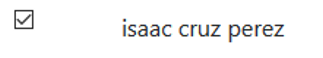
\includegraphics[scale=.5]{images/player_selected}} & \multicolumn{1}{l|}{}   & \multicolumn{1}{l|}{}   & \multicolumn{1}{X|}{}              \\ \hline

\end{tabularx}

\begin{tabularx}{\textwidth}{ X }
\multicolumn{1}{X}{\cellcolor[HTML]{9B9B9B}\textbf{Observaciones}} \\ \hline
\multicolumn{1}{|l|}{ }	\\
\multicolumn{1}{|l|}{ }	\\
\multicolumn{1}{|l|}{ }	\\
\multicolumn{1}{|l|}{ }	\\
\multicolumn{1}{|l|}{ }	\\
\multicolumn{1}{|l|}{ }	\\
\multicolumn{1}{|l|}{ }	\\
\multicolumn{1}{|l|}{ }	\\
\multicolumn{1}{|l|}{ }	\\
\multicolumn{1}{|l|}{ }	\\
\multicolumn{1}{|l|}{ }	\\
\multicolumn{1}{|l|}{ }	\\
\multicolumn{1}{|l|}{ }	\\
\multicolumn{1}{|l|}{ }	\\ \hline
\end{tabularx}
%===============================================================================================
\newpage

\subsection{P1-E1-CP10: Prueba de funcionalidad, caso de uso Eliminar equipo}

\begin{tabularx}{\textwidth}{ X l l X }
\multicolumn{4}{c}{\cellcolor[HTML]{9B9B9B}\textbf{Sistema: MTF}}                                                                                     \\
\multicolumn{4}{l}{\cellcolor[HTML]{EFEFEF}\textbf{P1-E1-CP10: Prueba de funcionalidad, caso de uso Eliminar equipo}}                                                   \\ \hline
\multicolumn{1}{|X|}{Pregunta}                               & \multicolumn{1}{l|}{Si} & \multicolumn{1}{l|}{No} & \multicolumn{1}{X|}{Observaciones} \\ \hline

\multicolumn{4}{|l|}{1. En la pantalla actual, \textbf{IU1.0 Pantalla de inicio del representante}, dé clic sobre el botón 
\includegraphics[scale=.3]{images/eliminate} del equipo}              \\
\multicolumn{4}{|l|}{recién actualizado.} \\ \hline
\multicolumn{1}{|X|}{1.1. ¿El sistema mostró el \textbf{IU2.2 Pantalla emergente para eliminar equipo}?} & \multicolumn{1}{l|}{}   & \multicolumn{1}{l|}{}   & \multicolumn{1}{X|}{}              \\ \hline

\multicolumn{4}{|l|}{2. Dé clic sobre el botón \IUbutton{Cancelar} }              \\ \hline
\multicolumn{1}{|X|}{2.1. ¿El sistema mostró la \textbf{IU1.0 Pantalla de inicio del representante}?} & \multicolumn{1}{l|}{}   & \multicolumn{1}{l|}{}   & \multicolumn{1}{X|}{}              \\ \hline

\multicolumn{4}{|l|}{3. Vuelva a presionar el botón 
\includegraphics[scale=.3]{images/eliminate} y dé clic sobre el botón \IUbutton{Si}}              \\ \hline
\multicolumn{1}{|X|}{3.1. ¿El sistema mostró el \textbf{MSG2.3 ''Equipo eliminado. Se ha eliminado a ESCOMIANOS correctamente''}?} & \multicolumn{1}{l|}{}   & \multicolumn{1}{l|}{}   & \multicolumn{1}{X|}{}              \\ \hline
\end{tabularx}

\begin{tabularx}{\textwidth}{ X }
\multicolumn{1}{X}{\cellcolor[HTML]{9B9B9B}\textbf{Observaciones}} \\ \hline
\multicolumn{1}{|l|}{ }	\\
\multicolumn{1}{|l|}{ }	\\
\multicolumn{1}{|l|}{ }	\\
\multicolumn{1}{|l|}{ }	\\
\multicolumn{1}{|l|}{ }	\\
\multicolumn{1}{|l|}{ }	\\
\multicolumn{1}{|l|}{ }	\\
\multicolumn{1}{|l|}{ }	\\
\multicolumn{1}{|l|}{ }	\\
\multicolumn{1}{|l|}{ }	\\
\multicolumn{1}{|l|}{ }	\\
\multicolumn{1}{|l|}{ }	\\
\multicolumn{1}{|l|}{ }	\\
\multicolumn{1}{|l|}{ }	\\ \hline
\end{tabularx}
%=================================================================================================

\end{document}
